\documentclass[12pt,a4paper,UKenglish]{article}
%\documentclass{article}
\usepackage{listings}
\usepackage[utf8]{inputenc}
\usepackage[T1]{fontenc,url}
\usepackage{babel,csquotes,newcent,textcomp}
\usepackage[backend=biber, maxbibnames=99]{biblatex}
\usepackage{graphicx}
%\bibliographystyle{unsrt}
%\usepackage{natbib}
%\bibliographystyle{unsrt}

\title{Essay on persistent memory}  % Declares the document's title.
\author{Svein Gunnar Fagerheim}      % Declares the author's name.
%\date{May 19, 2019}      % Deleting this command produces today's date.
\addbibresource{mini.bib}
%\bibliographystyle{unsrtnat}
\newcommand{\ip}[2]{(#1, #2)}

\begin{document}             % End of preamble and beginning of text.
\maketitle                   % Produces the title.

\section{Introduction}
High performance computing (HPC) is being used to analyze massive amount of data. Where the DRAM has always been a bottleneck to keep in mind when developing code to analyze the data. Persistent memory is changing this by providing cheap, fast and persistent memory that can store data even after a shut down.
This essay will explore where persistent memory is currently at, what are the advantages and challenges associated with persistent memory. And the essay will explore the different libraries that exist and possibly determine which one is best.

\subsection{What is persistent memory}
Persistent memory\cite{Rudoff2} is a non-volatile storage memory\cite{Mahmut} that is byte-addressable and has speed close to that of DRAM. DRAM stands for direct random-access memory, this is a volatile storage system that will lose all its data when the computer is shut down or restarted. Applications and data used by the CPU are temporarily loaded into memory from a hard drive in order to reduce latency and increase bandwidth. Persistent memory is another layer between the CPU and the disk. The data the CPU has the most use for is stored in the L1-L3 caches. When the cache is full the data needs to be evicted the evicted data will be sent back to the memory. If the data usage of the program is so large that it exceeds the memory available on the computer then the computer will start using virtual memory on the disk which is a lot slower then DRAM. The reason virtual memory is so slow is because one must do an I/O block to read and write to disk which takes time. Persistent memory is a layer between the DRAM and the disk in which the CPU can access directly just like it would do a normal DRAM. Figure 1 illustrates where in the hierarchy the persistent memory is placed.
\begin{figure}
	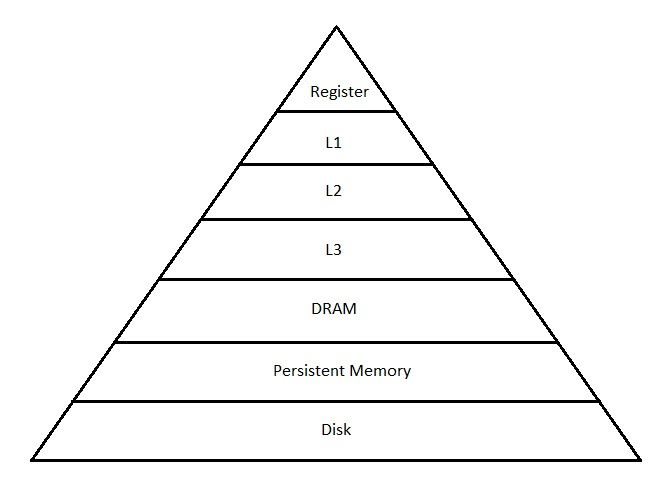
\includegraphics[scale=0.85]{Pyramid.jpg}
	\caption{Persistent memory becomes a new level between DRAM and Disk\cite{optane}}
	\label{fig:Pyramid}
\end{figure}

\section{Challenges}
\subsection{Consistent updates}
When writing data to storage that will persist even after a shutdown there must be a way to ensure that the data is either fully stored to the storage device or not at all. If there is an interruption taking place, for example power failure and the storage system does not have a way of ensuring that the data won’t be partially written to the storage device, then that will lead to corrupted data. Not only would the unsaved data the application was working on be lost, old data loaded into the application would also be lost if the application was in the process of overwriting old data with unsaved data\cite{Volos}. 
Traditional storage devices such as hard drive and SSD have several methods to ensure that the data won’t be corrupted by interruptions such as shadow updates, soft updates, journaling, and post-reboot checking. This is done automatically by the OS, so the programmer does not need to think about this. Since the application has direct access to the hardware, the programmers need to ensure that the application can perform consistent updates. 

\subsection{Security}
Another challenge when it comes to persistent memory is security and privacy\cite{Badam}. When an encryption key is used to unlock files, the key is stored in the memory. If it is DRAM then the key will disappear when the computer is shut down, but if it is stored in persistent memory it will persist and remain there until it is deleted. It will be very easy for someone to extract data from persistent memory if the person is able to gain access to it. The same concern also applies to personal information that is being stored in the persistent memory. When developing applications that will use persistent memory and handling sensitive information the programmer needs to remember that data he puts in persistent memory will stay there until it is deleted. It’s also worth mentioning that when the data is deleted or deallocated in the memory, the OS makes the space available to another application. The data is only deleted when its overwritten.

\subsection{Durability}
Another challenge for persistent memory is durability. While persistent memory behaves more like DRAM it still has a considerably shorter lifespan than DRAM\cite{Badam}. This is because persistent memory can only write data to a certain amount of time to a region before the region can no longer hold any data reliably. While the storage capacity of persistent memory has increased, so has the bit error rate increased even more. The solution to this is to either have the hardware mask all the regions with bit error from the software or have the hardware expose them to the software and let the software handle the rest. There is also the possibility of letting the hardware and software work together in order to mask regions with bit errors. This will expand the lifespan of persistent memory, but the challenge for hardware producers is to come up with new technologies that can increase the durability of the persistent memory.

\subsection{Persistent memory leaks}
A common problem one might have when programming in C are memory leaks. When the application is using normal DRAM, the memory consumed by the application can be freed just by restarting the application. If the application is using persistent memory on the other hand, then the memory consumed by the application will remain consumed even after the program has been restarted.\cite{Volos}\cite{Swanson} Memory leaks will persist a shutdown just like persistent memory will. The technology must ensure that the memory occupied on the persistent memory can be tracked down to the application that allocated the memory. By doing this it is possible to track down and remove memory leak for the persistent memory.

\subsection{Programming challenges}
When handling a massive amount of simulation data there will be a few challenges when it comes to programming with persistent memory. One challenge is how to decide where the data will be stored, either in DRAM or persistent memory when the simulation data are coming in. There is also the question when to transfer data from persistent memory to DRAM and when to evict data from DRAM. The transfer of data between DRAM and persistent memory will also take up CPU that could have been used on other things. This means that sometime it might be cheaper for the CPU to work data from the persistent memory instead of transferring it to DRAM first. 
\newline\newline
%\subsection{Flow of data}
Another challenge would be how to manage the flow of simulation data that will come in. The first step in managing the data would to decrease the size of raw data. This can be done by separating the data that is considered interesting and throw away the rest. The relevant data might be identified by a pattern in the data that comes in. 
\newline\newline
%\subsection{Analyzing data}
In this project the data will be analyzed while it comes flowing in. There is a trade off between speed and how much the data can be analyzed. Analyzing data takes CPU away from managing the flow of data and if the management of data does not happen fast enough in order to keep up with the incoming data.

\section{Advantages}
\subsection{Cost}
One of the biggest shortcomings of DRAM is that it is expensive. When the amount of memory increases in a system the cost of DRAM scales nonlinearly.\cite{Badam} This has led to memory becoming a bottleneck in servers that runs programs where a lot of memory is needed. Persistent memory is more scalable in terms of cost then compared to DRAM. 

This will enable servers to have more storage capacity that can be read at almost the same speed as DRAM.

\subsection{Capacity, Larger physical memory}
The memory capacity of persistent memory represents a drastic increase in the size of memory that is available to the user. The biggest size of a DRAM memory module that can be bought today is 64 Gigabytes. Intel has announced a new persistent memory called Intel Optane DC\cite{side1}. This is a persistent memory that is compatible with a DDR4 socket and each memory module can contain 512 Gigabytes of memory. The bigger memory size will make it possible to keep more of the data the user is working on in the memory and reduce the traffic between the memory and the hard drive.

\subsection{Byte addressable, low latency}
Since the persistent memory is connected to a DRAM slot it is also byte-addressable. When a program accesses traditional storage it must wait for the OS to do an I/O block in order to get access which takes a long time and read/write are done in 4 kB blocks. With persistent memory the program can skip the I/O block and access the data directly, this will dramatically decrease the latency. Typical latency when using DRAM would be around 10\textsuperscript{-7}\cite{lerebok} while Intel has measured their Optane DC to have a latency of 4.1 ms\cite{optane2}. Persistent memory is 40 times slower than normal DRAM, but it is still a lot better than SSD that can have 80 ms latency. 

\section{Libraries}
Persistent memory makes it possible to dramatically decrease the latency that occurs when accessing a normal SSD. After the introduction of persistent memory, Windows and Linux have developed a new storage system for their OS that they call Direct Access or DAX. This storage system allows the programmer to bypass the traditional storage system and access the persistent memory directly\cite{Rudoff}. The new storage system can’t be taken advantage of by using traditional pointers, they will always use the traditional storage system. The programmer needs to use a new type of pointes that makes it possible for the program to access the persistent memory directly.

\subsection{SNIA}
Storage Networking Industry Association is a global non-profit organization that has a mission to “lead the storage industry worldwide in developing and promoting vendor-neutral architectures, standards, and educational services that facilitate the efficient management, movement, and security of information.” Many of the big tech companies such as Intel, Microsoft and Samsung are members of this organization and they have voting power. They work together to produce new standards when it comes to storage. 
\newline\newline
Today there already exist several open source libraries that can be used. Intel has an open source project called “Persistent Memory Development Kit” that can be found of the webpage pmem.io. The PMDK is a collection of different libraries that have been built upon the Direct Access system mentioned earlier, it will allow program access the persistent memory as memory-mapped files. PMDK is a vendor-neutral library that works on all persistent memory hardware that follows the SNIA NVM programming model. 

\subsection{Libpmem}
This is the most basic library in the PMDK. It provides a low-level support for persistent memory that the other libraries build upon. Libpmem\cite{libpmem} keeps track of what kind of flush instruction the CPU support. The library does not have interfaces that handles transaction like the other libraries. The programmer must create code for doing transaction that can handle interruptions. The transactions must be able to either transfer the data fully or not at all in the case of interruptions. The team that created this library suggested that the programmer will end up changing library or “steal” code from the other libraries just because of how tedious it is to develop their own code that can handle the detection of supported instructions and other things the code must be able to handle.

\subsection{Libpmemobj}
Libpmemobj\cite{libpmemobj} allows objects to be stored in persistent memory without being torn by interruptions. The objects in question are not class objects one finds in C++, but instead they are variable-sized blocks of data that fall under the term object storage. The object has an object ID that is independent when it comes to location. The changes or updates to these objects are atomic because the library have transactions to make this happen. This library can be used for multithreading and are have been optimized for scaling when it comes to multithreading. The main author also mention that the C++ version of this library is the cleanest and least prone to error compared to all the other libraries\cite{Rudoff}. He therefore recommends that programmers should start using this library if they are new to persistent memory programming. 

\subsection{libpmemblk and libpmemlog}
These libraries are made for specific cases. 
libpmemblk\cite{libpmemblk} is used for handling large arrays of persistent memory blocks. The blocks must be larger than 512 bytes in order to work. This library is useful if the program is made to manage a block cache. Libpmemlog\cite{libpmemlog} is used to append log files. If the program logs a lot of data, it might be better to use libpmemlog in order to avoid going through the traditional file system where most of the time would be spent waiting. 
Both libraries are built upon the libpmem library, but unlike libpmem their updates can’t be torn because of interruptions.

\subsection{libmemkind}
Libmemkind\cite{libmemking} is the successor of the libvmem\cite{libvmem} library which is now deprecated. The libmemkind is for programs where the programmer doesn’t care about persistency. It supports the traditional allocations and deallocation of memory with the functions \texttt{memkind\_malloc} and \texttt{memkind\_free}. The advantage of the libmemkind library is that it will use the persistent memory as a second layer of DRAM. Since persistent memory is a lot cheaper per GB of memory than DRAM. The disadvantage is that persistent memory is still a little slower than DRAM so computation will take a little longer.

\subsection{libvmmalloc}
The libvmmalloc\cite{libvmmalloc} library is almost the same as the libmemkind. The difference is that the memory pool is automatically created and destroyed every time a process is created of terminated. Another difference is that the memory pool replaces the system heap. The advantages of this is that there is no need to change anything in the code other than importing the libvmmalloc library. The disadvantage is that the code now only uses persistent memory and never DRAM. This will slow down to a certain degree. 

\subsection{librpmem}
The librpmem\cite{librpmem} library can access the persistent memory remotely using the RDMA protocol. The library uses an SSH connection to authenticate the user before allowing access to the persistent memory. Because of the distance between the computer and the data this library will be very slow when computing large amount of data. This library is still considered an experimental API.

\subsection{The rest}
Pmem.io has several other libraries on their webpage. Libpmempool and pmempool are for management, diagnostic, and repair of memory pool. There is also libvmemcache which is used for volatile key-value stores.

\subsection{Which library?}
Analyzing data has traditionally been done in a two-step process. First the raw data is being collected and stored on a file and only when all the data has been collected will it be analyzed by another application. This process is time-consuming because it takes a long time to store and read data from a hard drive. With the increasing amount of data being created because of improvements of data gathering tools, this problem will only increase in the future. This project is about creating an application that can analyze simulation data “in-situ” as soon as the simulation data are being generated. The goal by doing this is to decrease the amount of raw data that must be stored on a file and decrease the time consumption for the process.
\newline\newline
The libpmemblk and libpmemlog, can easily be ruled out since the project will be one big persistent memory block instead of many small ones and there will be no need of logging the activity that happens. Librpmem can also be ruled out since the remote access to persistent memory will be too slow. The libpmem is a very basic library and most likely unsuited for this project since the author of the library mentions that the user must make their own algorithm in order to make it work. This would be time consuming for this project and since the benefit in terms of performance for making custom functions will most likely be small. 
\newline\newline
Libpmemobj is the most versatile of all the libraries available and will most likely be the best choice for developers when it comes for implementing persistent memory. This is a library that focuses on ensuring that data is being stored on persistent memory without being teared because of interruptions. This is unnecessary for this project because persistent memory will be used to store data temporarily until it can be processed by the analyzing application. If an interruption takes place it would mean that data gathering will come to an end must be restarted, therefore there is no need for the data to be persistent. 
\newline\newline
The library best suited for the project would be either the libmemkind or the libvmmalloc. The reason for this is because the data will only be stored in the persistent memory temporarily. The libraries will behave just like an ordinary DRAM would, but at a slightly slower speed than real DRAM. Since libvmmalloc only makes use of persistent memory and not DRAM it is less suitable for this project because not making use of the faster DRAM will make the the application to slow.
\newline\newline
Below is an example of how persistent memory can be used. When allocating an array to persistent memory one must specify what kind of memory to allocate. In this example \texttt{MEMKIND\_DEFAULT}\cite{memkindlib} was used, this means that the program uses standard memory and default page size. There is also a chance that persistent memory will not be allocated, in that case \texttt{MEMKIND\_DEFAULT} will return NULL.
\lstset{language=C}
\begin{lstlisting}
#include <stdlib.h>
#include <memkind.h>

int main(int argc, char **argv){
  int i;
  //Allocation to DRAM
  int *p = (int*)malloc(10*sizeof(int));
  for(i=0; i<10; i++){
    p[i]=i;
  }
  
  //Allocating an array to persisten memory.
  int *array = (int*)memkind_malloc(
      MEMKIND_DEFAULT, 10*sizeof(int));
  if (array == NULL) {
    printf("\nAllocation Failed!");
    return 0;
  }
	
  //Transfers array from DRAM to persisten memory.
  for(i=0; i<10; i++){
    array[i] = p[i];
  }
  
  //Deallocate both arrays.
  memkind_free(MEMKIND_DEFAULT, array);
  free(p);
	
  return 0;
}
\end{lstlisting}

\nocite{*}
%\nocite{*}
%\bibliographystyle{unsrt}
\printbibliography


\end{document}               % End of document.
